\documentclass{article}
\usepackage[left=2cm,right=2cm,top=2cm,bottom=2cm]{geometry}
\usepackage[utf8]{inputenc}
\usepackage[german]{babel}
\usepackage{amsmath}
\usepackage{dsfont}
\usepackage[export]{adjustbox}
\usepackage{amsthm}
\usepackage{color}
\usepackage{amsfonts}
\usepackage{amssymb}
\usepackage{wasysym}
\usepackage{makeidx}
\usepackage{graphicx}
\usepackage[colorlinks=true,urlcolor=blue,linkcolor=blue]{hyperref}
\usepackage{ziffer}
\usepackage{minted}
\usepackage{xcolor}
\usepackage{framed}
\usepackage{mdframed}
\usepackage{subfiles}
\usemintedstyle{emacs}

\definecolor{purp}{HTML}{9A72AC}
\definecolor{re}{HTML}{FC6255}
\definecolor{gre}{HTML}{83C167}
\definecolor{blu}{HTML}{58C4DD}
\definecolor{shadecolor}{rgb}{0.85,0.85,0.85}
\definecolor{bg}{rgb}{0.95,0.95,0.95}
\setlength{\parindent}{0em} 

\BeforeBeginEnvironment{minted}{\begin{mdframed}[linewidth =2 ,backgroundcolor=bg , linecolor=black, linewidth=0.5]}
\AfterEndEnvironment{minted}{\end{mdframed}}

\newtheorem{defi}{Definition}
\BeforeBeginEnvironment{defi}{\begin{mdframed}[linewidth =2 ,backgroundcolor=bg , linecolor=black, linewidth=0.5]}
\AfterEndEnvironment{defi}{\end{mdframed}}

\newcommand{\bsp}{\textbf{Beispiel}:}
%\newcommand{\task}{\textbf{Aufgabe}:}

\newcommand{\bol}[1]{\textbf{#1}}
\newcommand{\q}[1]{\glqq #1\grqq}
\newcommand{\DODO}[1]{\textbf{\textcolor{red}{DODO:}} #1 \\ \begin{center}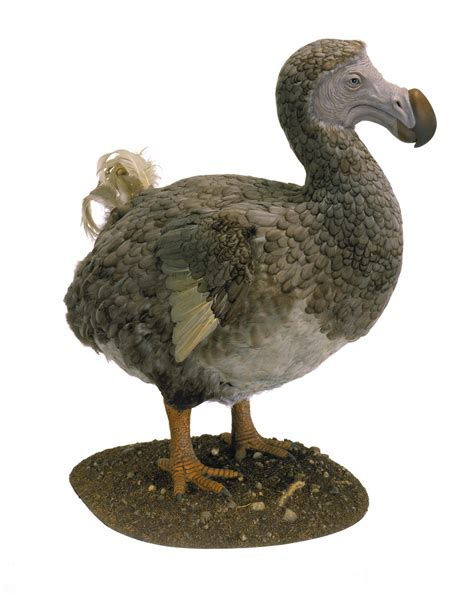
\includegraphics[scale=0.2]{../../media/dodo.jpg} \end{center}}

\newenvironment{task}[1]{
    \begin{shaded*}
    \textbf{Aufgabe #1}:
}{
    \end{shaded*}
}



\begin{document}

\subsection{Grundbegriffe}

Die Idee des Baumes in der Informatik wurde sogar schon in der 6. Jahrgangsstufe behandelt! Zur Auffrischung: \\
Ein Baum besteht aus \bol{Knoten} (nodes) und \bol{Kanten} (edges). Je nachdem, wo diese Knoten liegen unterscheidet man noch zwischen der \bol{Wurzel} (root), den \bol{inneren Knoten} (inner node) und den \textbf{Blättern} (leaves).
\begin{center}
    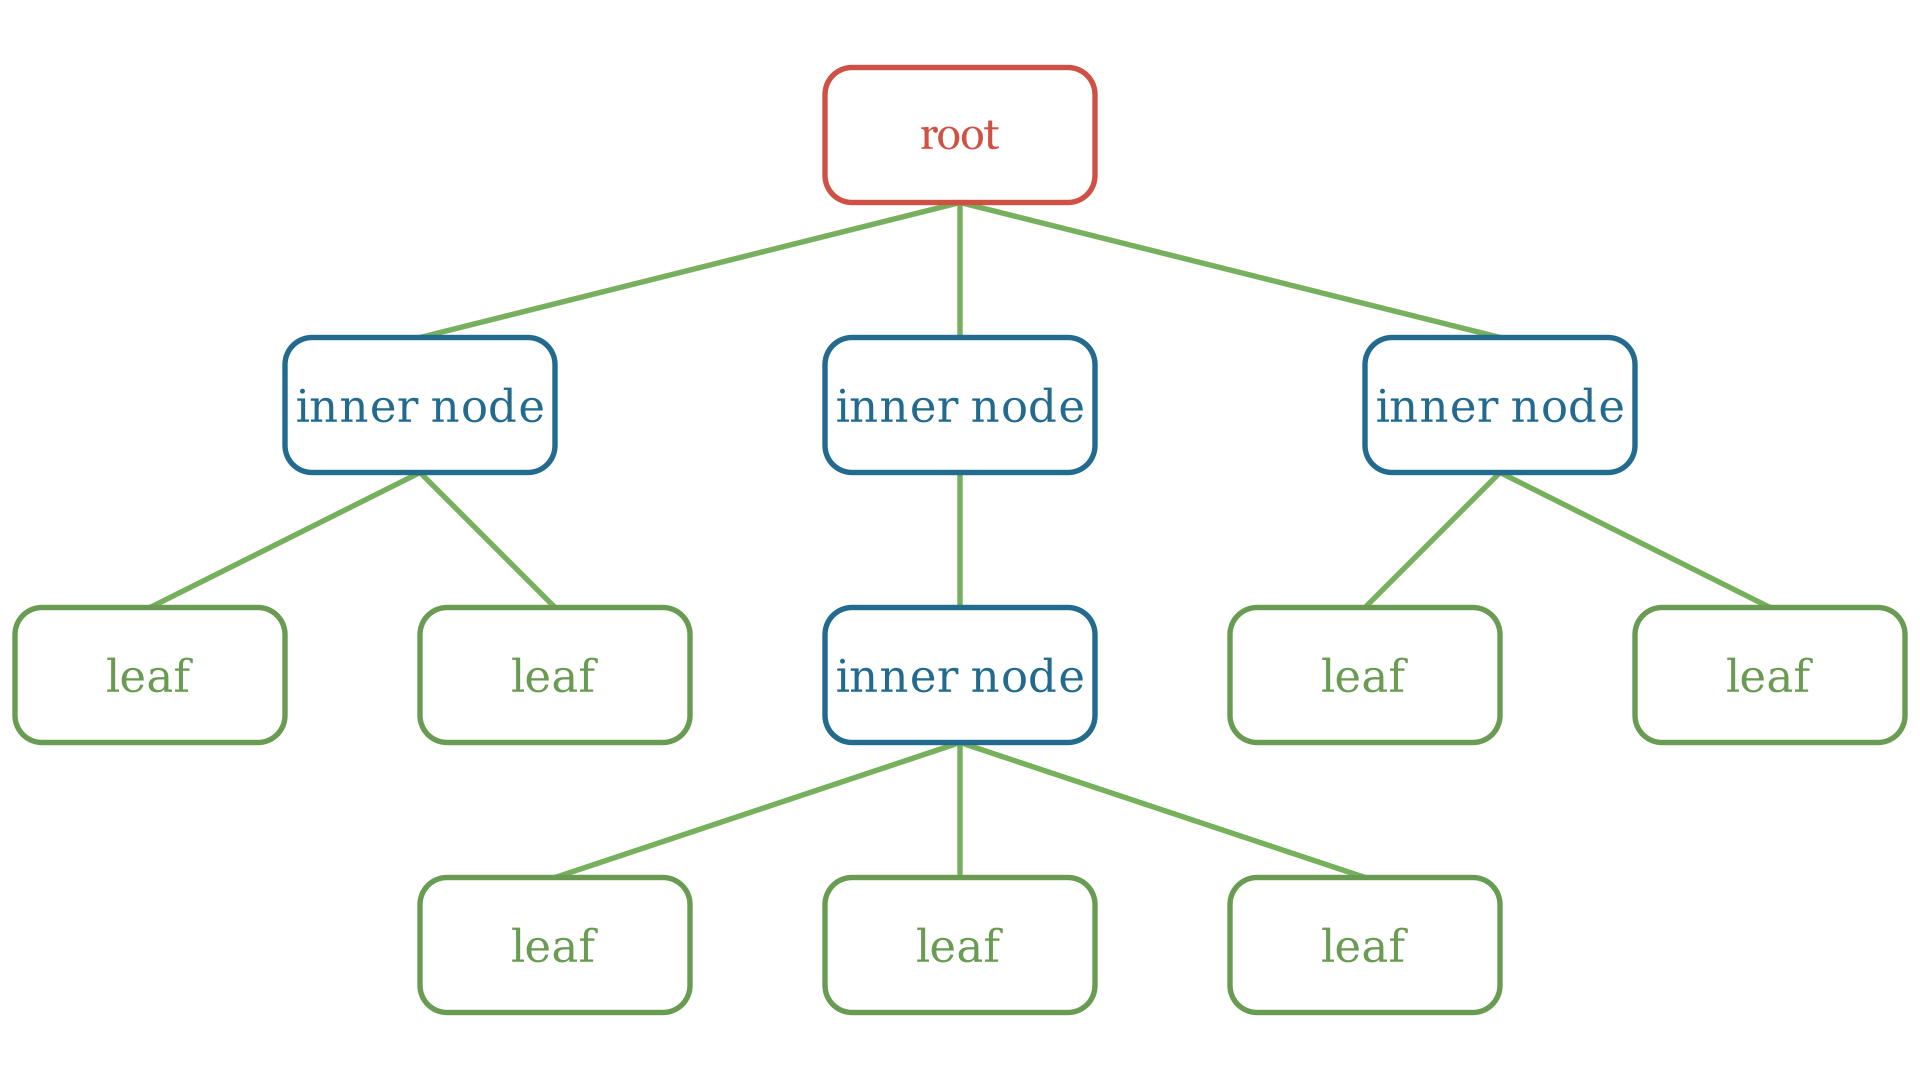
\includegraphics[scale=0.2]{../../media/tree_example.png}
\end{center}
Schon die optische Betrachtung dieser Struktur vermittelt den Eindruck, das auch hier mit einer verzeigerten Struktur gearbeitet werden kann. Ähnlich wie bei der Liste gibt es eine steuerende Klasse \textbf{Baum} bzw. \textbf{Tree}, die für den Aufruf von Methoden auf der Wurzel zuständig ist. \\
Im Gegensatz zur Liste hat die Wurzel jetzt mehrere Nachfolger, man spricht hier auch von \textbf{Kindknoten} (\textbf{child Node}) und \textbf{Elternknoten} (\textbf{parent nodes}). \\
Bevor die konkrete Implementierung eine Rolle spielt, zunächst ein Beispielbereich der Informatik, in dem eine Baumstruktur sehr häufig vorkommt, die \textbf{Suche}. Dabei beschränken wir uns der Einfachheit halber zunächst auf Bäume, die \textbf{soritert} und \textbf{binär} sind, d.h. jeder Knoten kann maximal zwei Kinder haben.

\subsection{Die Suche nach einer Zahl}

Wir nehmen an, dass bereits eine sortierte Liste an Zahlen vorliegt, z.B.:
\begin{center}
    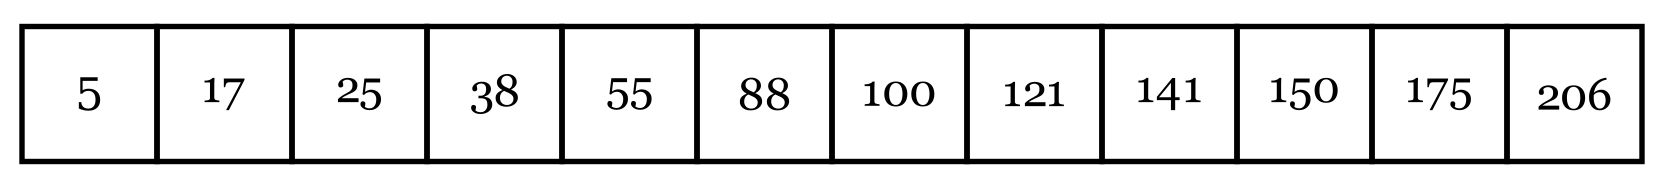
\includegraphics[scale=0.25]{../../media/search.png}
\end{center}
Die Suche nach einer gegebenen Zahl, z.B. $100$ wurde bereits für die Array List und für die Linked List implementiert. In beiden Fällen besteht die grundlegende Idee darin, sich die Liste, entlangzuhangeln und an jedem Knoten (bzw. an jedem Platz im Array) zu vergleichen, ob die Zahl an dieser Stelle sitzt (für die Linked List ist dies auch in Ordnung so!).
\begin{center}
    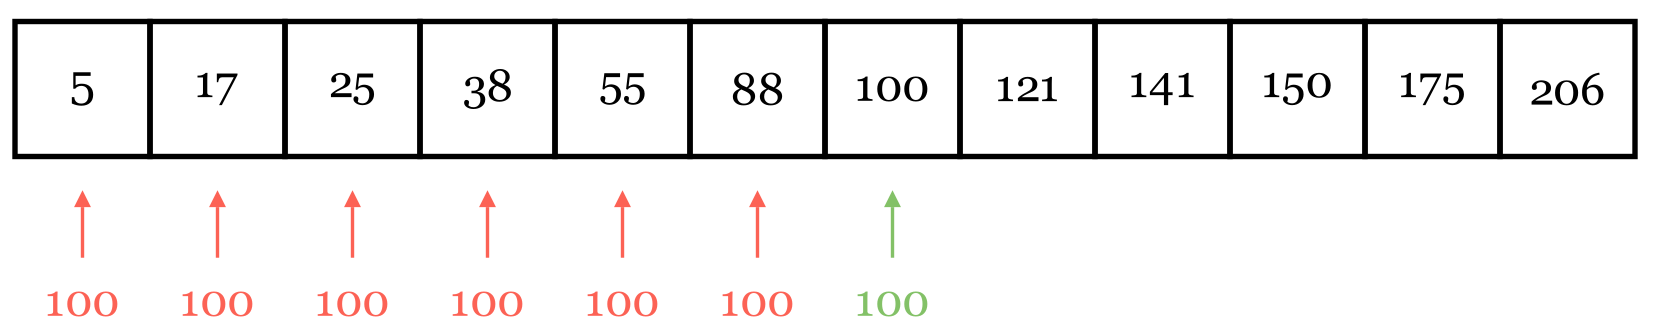
\includegraphics[scale=0.25]{../../media/search2.png}
\end{center}
Ist die Liste sortiert können wir zumindest noch eine Verbesserung der Performance erreichen, indem wir den Suchalgorithmus abbrechen lassen, sobald er eine Zahl erreicht, die größer als die gesuchte Zahl ist. Finden wir die Zahl, so können wir ohnehin abbrechen.\\
Im schlechtesten Fall (engl. Worst-Case) müssen wir aber dennoch die gesamte Liste durchlaufen und jedes einzelne Element mit unserer Eingabe vergleichen. In Bezug auf die \textbf{Laufzeit} unseres Algorithmus ist dies sicher nicht ideal, man spricht hier von einer linearen Laufzeit, oder kurz, der Algorithmus ist in $\mathcal{O}(n)$ (Details zur sogenannten $\mathcal{O}$-Notation für Interessierte im Anhang!). \\
Würde ein Mensch diese Suche übernehmen, so würde er sicher nicht schrittweise vergleichen, wenn bekannt ist, dass die Liste sortiert ist. Wir gehen der Einfachheit halber davon aus, dass für unseren Menschen die Liste als \q{Buch} vorliegt, bei dem auf jeder Seite eine Zahl steht. Ein typisch \q{menschliches} Suchmuster sähe algorithmisch etwa so aus:
\begin{minted}{Java}
    Schlage das Buch etwa in der Mitte auf 
    wiederhole solange die Zahl nicht gefunden ist:
        Ist die abgebildete Zahl größer als die gesuchte Zahl:
            Suche im "linken" Bereich des Buches weiter
        sonst:
            Suche im "rechten" Bereich des Buches weiter 
\end{minted}
Für die Suche im \q{linken} bzw. \q{rechten} Bereich kann ebenso wieder die Strategie des \q{in der Mitte}- Aufschlagens verwendet werden. Ist man nahe an der gesuchten Zahl wird ein Mensch vermutlich auch beginnen einfach zu blättern.\\
In jedem Fall ist dieses Vorgehen effizienter als das bloße Durchgehen der Liste nach der Reihe, es ist eine \q{intelligentere} Form des Suchens. \\
Wir betrachten wieder das Beispiel von oben und suchen diesmal die Zahl 150. Die Suche startet aber diesmal in der Mitte,  d.h. beim $6-$ ten Eintrag unserer Liste , hier: 88. \\
(\textit{Hinweis}: man könnte auch den Siebten Eintrag als Mitte definieren, bei geraden Anzahlen an Elementen kann auf- oder abgerundet werden, das spielt im Prinzip keine Rolle!)
\begin{center}
    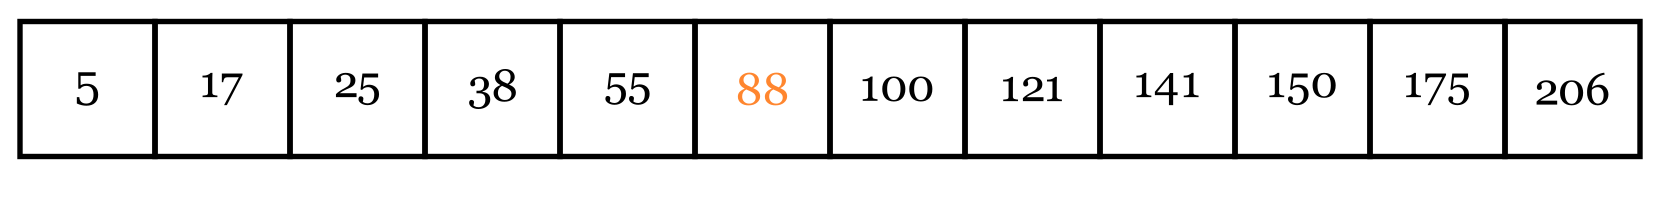
\includegraphics[scale=0.25]{../../media/search3.png}
\end{center}
Damit ist klar, dass die Zahl rechts der 88 liegen muss, die 5 Zahlen links der 88 kann ich sofort ausschließen, wir suchen uns wieder die Mitte der verbleibenden 6 Zahlen, also die 3. Zahl, in diesem Fall 141:
\begin{center}
    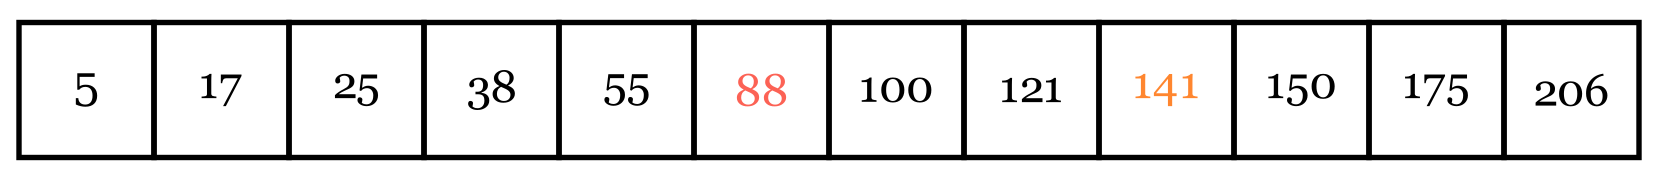
\includegraphics[scale=0.25]{../../media/search4.png}
\end{center}
Da 141 immer noch kleiner als 150 ist, betrachten wir wieder den rechten Bereich und im nächsten Schritt wird mit der 175 verglichen:
\begin{center}
    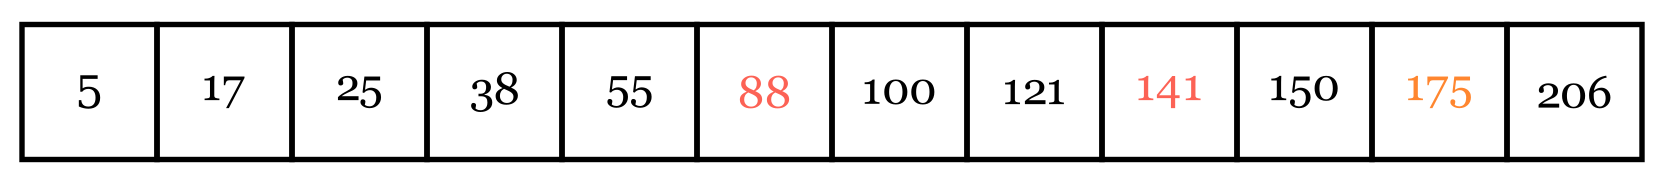
\includegraphics[scale=0.25]{../../media/search5.png}
\end{center}
Zum ersten Mal sind wir zu groß! D.h. wir müssen den linken Bereich betrachten, dieser ist jetzt aber nur noch ein Element groß! D.h. wir haben in diesem Fall die 150 gefunden:
\begin{center}
    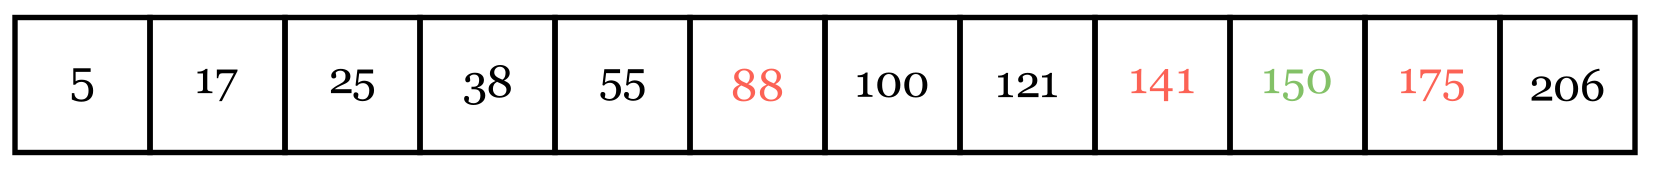
\includegraphics[scale=0.25]{../../media/search6.png}
\end{center}
Insgesamt hat in dieser Variante also bereits der vierte Vergleich zum Erfolg geführt, in einer linearen Implementierung wären dagegen zehn Vergleiche notwendig gewesen.\\
Um eine bessere Analyse des Aufwands zu erhalten, muss der durchschnittliche Suchaufwand (engl.: Average Case) betrachtet werden, um auszuschließen, dass wir in diesem Fall einfach nur \q{Glück} hatten. \\
Um mathematisch etwas aussagen zu können, gehen wir der Einfachheit halber davon aus, dass alle Positionen für eine Zahl im Array gleich wahrscheinlich sind- das ist im Allgemeinen keine starke Einschränkung, wenn wir nichts über die Anzahl an Zahlen und Verteilungen wissen. In unserem Beispielarray mit 12 Einträgen hat eine zu suchende Zahl also eine Wahrscheinlichkeit von jeweils $\frac{1}{12}$ an einer bestimmten Stelle zu sein. \\
Im besten Fall finden wir gleich beim ersten Vergleich unsere Zahl, im schlechtesten Fall (engl.: Worst Case) nach zwölf Vergleichen. Jede dieser Möglichkeiten hat aber die gleiche Wahrscheinlichkeit, deswegen können wir rechnen:
\begin{center}
    $\frac{1}{12}\cdot 1 + \frac{1}{12} \cdot 2 + \dots + \frac{1}{12} \cdot 11 + \frac{1}{12} \cdot 12 = \frac{1}{12} \cdot (1+\dots + 12) = \frac{1}{12}\cdot 78 = 6,5$
\end{center}
Im Schnitt werden bei der \textbf{linearen Suche }also $6,5$ Vergleiche gebraucht, um einen Eintrag zu finden.
\vspace{2mm}
Zurück zu unserer \textbf{menschlichen Suche} (der Fachbegriff dafür in unserem Kontext ist eigentlich \textbf{binäre Suche} oder englisch \textbf{binary search}). Im Besten Fall finden wir auch hier nach genau einem Schritt die Lösung (wenn wir die 88 suchen würden), der schlechteste Fall (wie die 150) braucht aber nur 4 Schritte! Hätten wir beispielsweise nach \textbf{149} statt 150 gesucht, so wäre auch nach diesem vierten Vergleich die Suche beendet, da wir bereits mit der nächstkleineren Zahl, nämlich 141 verglichen hatten. \\
Um den durchschnittlichen Aufwand zu bestimmen kann bestimmt werden, nach wie vielen Schritten jede Zahl erreichbar ist:
\begin{center}
    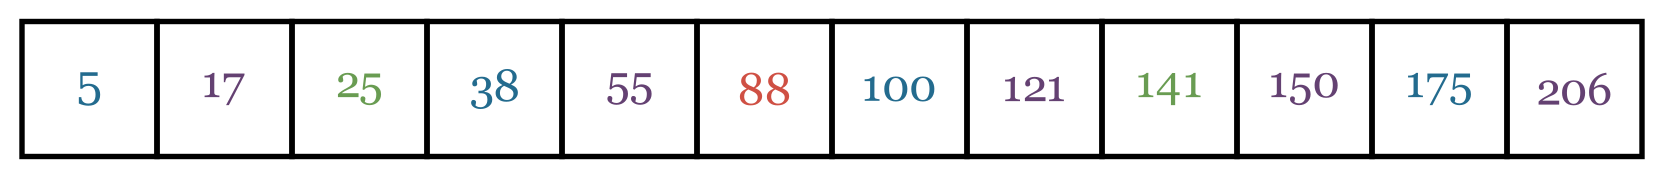
\includegraphics[scale=0.25]{../../media/search7.png}
\end{center}
Es werden:
\begin{itemize}
    \item Eine Zahl braucht \color{re}einen Vergleich\color{black}
    \item zwei Zahlen brauchen \color{gre}zwei Vergleiche\color{black}
    \item vier Zahlen brauchen \color{blu}drei Vergleiche\color{black}
    \item fünf Zahlen brauchen \color{purp}vier Vergleiche\color{black}
\end{itemize}
Damit ergibt sich:

\begin{center}
    $\frac{1}{12} \cdot (1\cdot 1+ 2\cdot 2+4\cdot 3 + 5\cdot 4) \approx 3,1$
\end{center}
Hier brauchen wir nur noch $3,1$ Vergleiche im Schnitt. Die Verbesserung wird noch deutlicher, wenn wir große Mengen an Daten betrachten. Dazu aber später bei der Implementierung der Suchmethode mehr! \\

\subsection{Vorüberlegung zur Implementierung}
Grundsätzlich können Bäume auch in Arrays eingebettet werden, im vorherigen Kapitel haben wir z.B. die binäre Suche auch innerhalb eines Arrays ausgeführt. Dabei haben wir schon eine Baumstruktur ausgenutzt (dazu später mehr). Für die eigentliche Suche kann eine Repräsentation im Array sogar vorteilhaft sein. Eine übliche Einbettung funktioniert dabei wie folgt (i für Index, v für value):

\begin{center}
    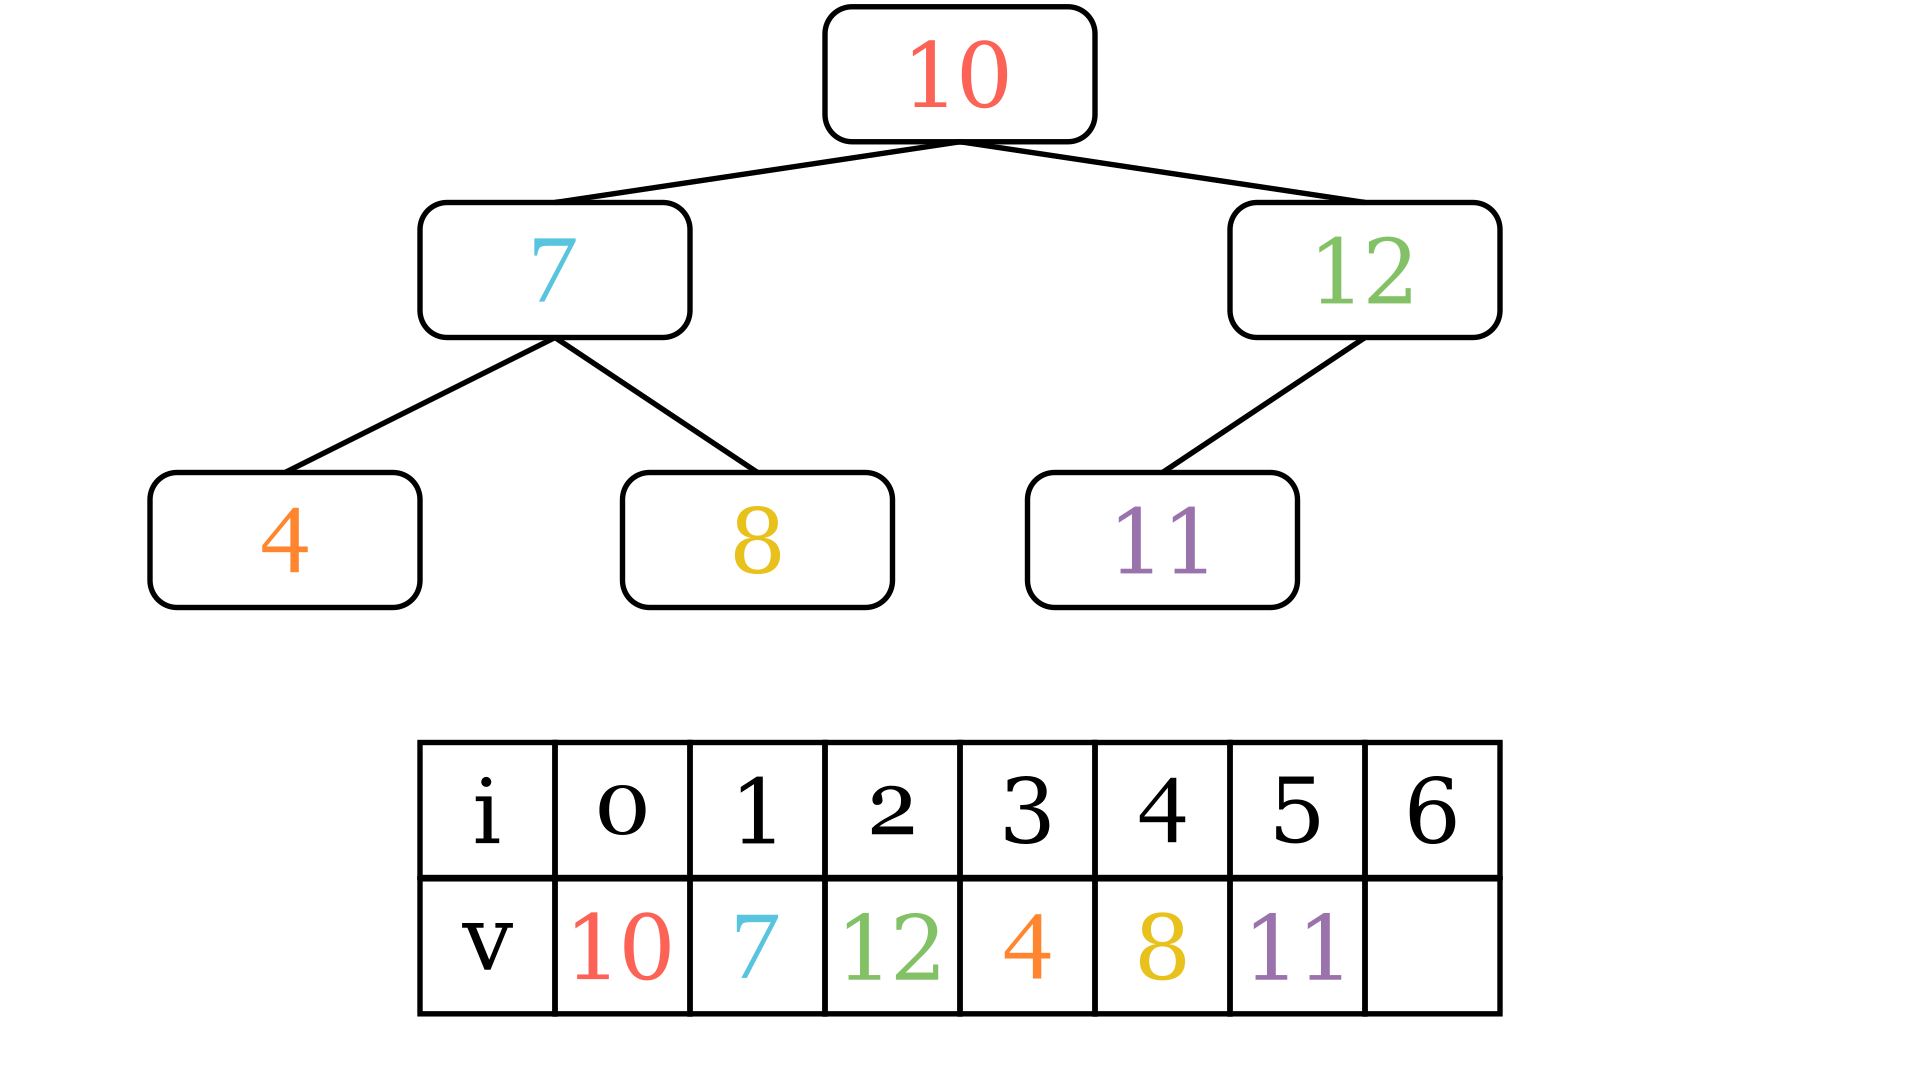
\includegraphics[scale=0.15]{../../media/einbettung.png}
\end{center}
Die Wurzel liegt beim nullten Index des Arrays, in den folgenden zwei Einträgen sind die beiden Kinder platziert, in den nächsten vier Einträgen dann die vier Enkel, u.s.w.. \\
Möchte man den Baum häufig vergrößern oder verkleinern (sprich Elemente hinzufügen oder Entfernen), so ergeben sich die selben möglichen Probleme wie bei der ArrayList! Ist der Baum darüber hinaus nicht \textbf{balanciert}, so ergeben sich viele Leerstellen. \\
Grob gesprochen ist ein Baum dann (aus)balanciert, wenn jede Reihe möglichst voll gefüllt ist. Der obige Baum ist beispielsweise gut balanciert. Dagegen wäre der folgende Baum sehr schlecht balanciert: 
\begin{center}
    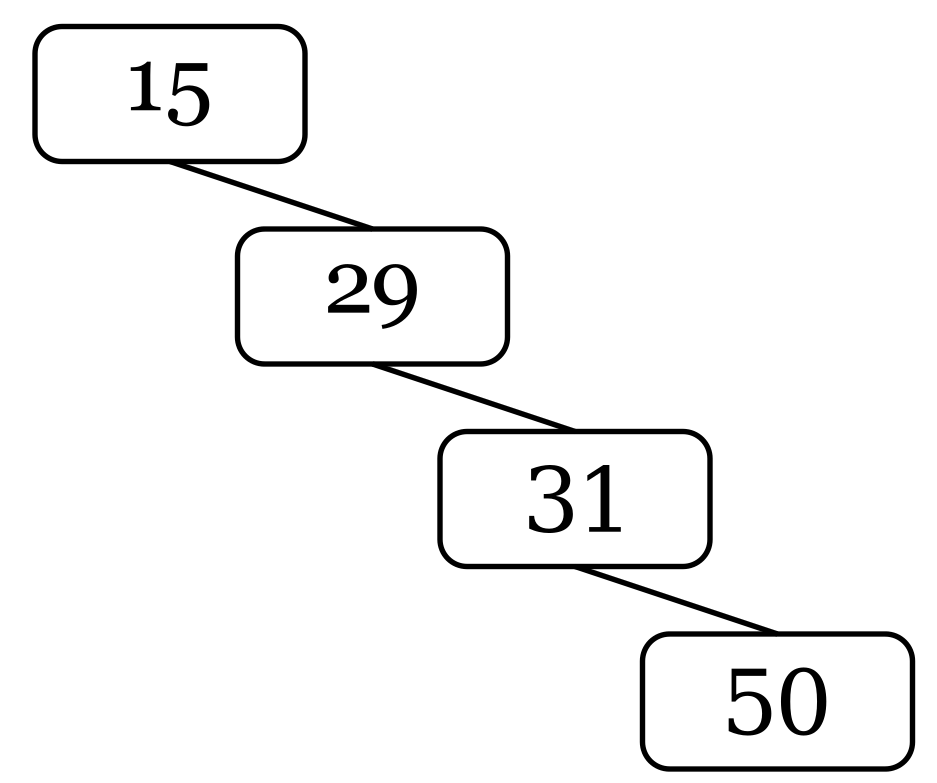
\includegraphics[scale=0.15]{../../media/linear.png}
\end{center}
\vspace{1mm}

Eine andere Möglichkeit ist ein Wurzelelement - also sinnvollerweise das Element, das bei einer Suche als erstes ausgespuckt wird (in unserem Beispiel von oben also die 88) - direkt auf die weiteren Elemente verweisen, die im nächsten Suchschritt verwendet werden. Von diesem Elementen verweisen wir anschließend wieder auf die nächsten Elemente in der Suchreihenfolge, usw. \\
Dadurch ergibt sich automatisch die Struktur eines Baumes (wie in den Zeichnungen oben schon angedeutet!). In diesem Fall hat jeder Knoten bis zu zwei Kinder:
\begin{itemize}
    \item der Knoten im linken Teilbaum, der verwendet wird, wenn das zu suchende Objekt \q{kleiner} als das Objekt im Knoten ist.
    \item der Knoten im rechten Teilbaum, der verwendet wird, wenn das zu suchende Objekt \q{größer} als das Objekt im Knoten ist.
\end{itemize}
Dadurch ergibt sich auch direkt eine Möglichkeit einen binären Baum aufzubauen: bei jedem einzufügenden Element hangelt man sich am Baum entlang und wählt - abhängig vom einzufügenden Element nach obigen Kriterien - den linken oder rechten Teilbaum vom derzeitigen Knoten aus gesehen. Ist an der gewählten Seite noch kein Knoten wird dieser eingefügt. \\
Der Baum aus dem obigen Einbettungsbeispiel kann also beispielsweise so entstanden sein: 
\begin{center}
    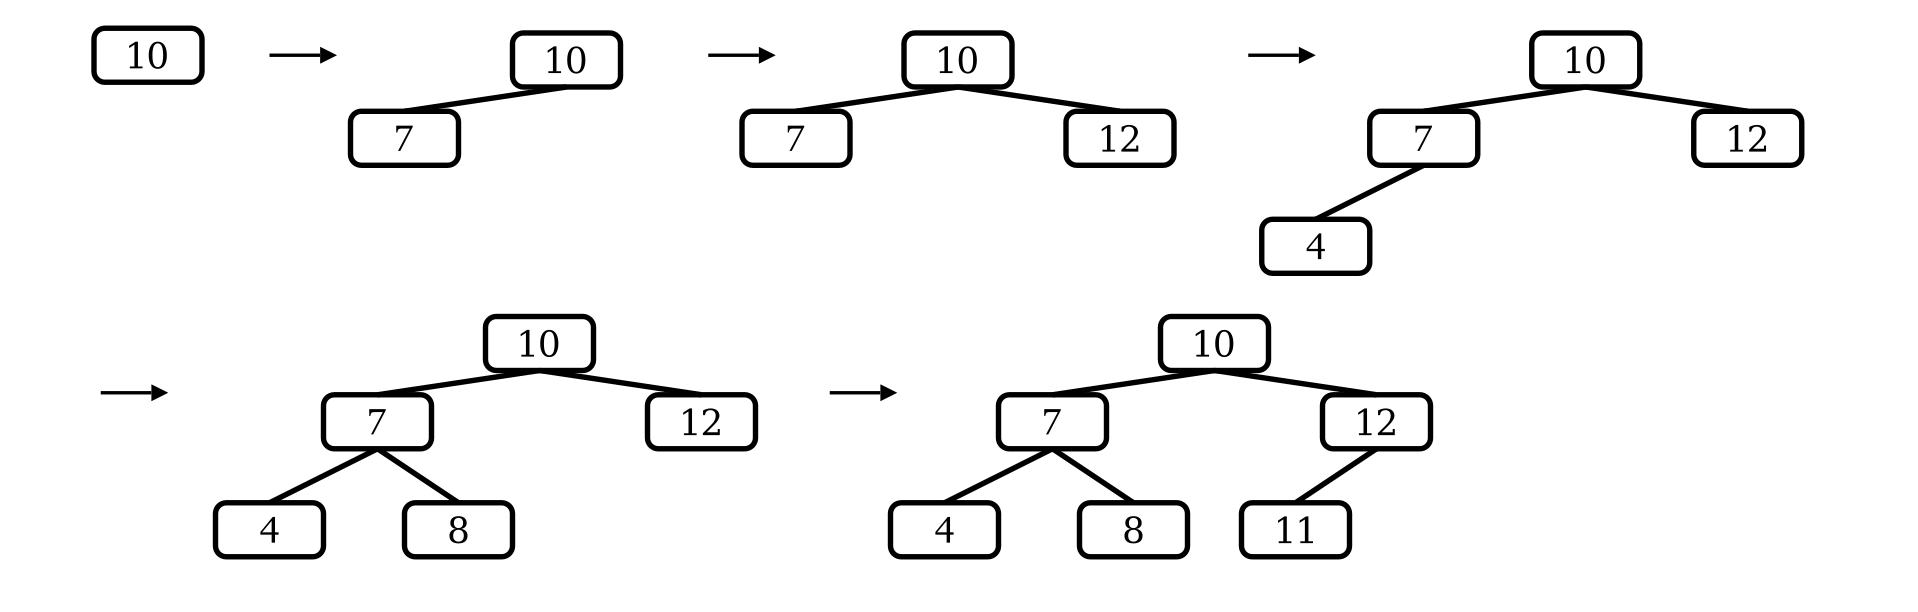
\includegraphics[scale=0.26]{../../media/insertExample.png}
\end{center}
\textit{Hinweise:}
\begin{itemize}
    \item größer und kleiner bezieht sich dabei nicht notwendigerweise auf Zahlen. Wie bei unserer Liste können wir auch nach anderen Kriterien ordnen. Solange der Vergleich zweier Elemente mit dieser Methode immer ein eindeutiges Ergebnis liefert (also größer, kleiner oder gleich) können beliebige Datentypen verwendet werden.
    \item Die sich ergebende Struktur des Baumes hängt natürlich von der Reihenfolge des Einfügens in den Baum ab. Hat die Wurzel beispielsweise den Wert $20$, wird die Zahl $22$ in den rechten Teilbaum eingefügt. Hat sie dagegen den Wert $25$, so wird $22$ in den linken Teilbaum eingefügt. \\
          Dadurch kann sich auch ein \q{Ungleichgewicht} ergeben. Am \q{schlechtesten} ist dabei ein Einfügen in bereits sortierter Reihenfolge:
          \begin{center}
              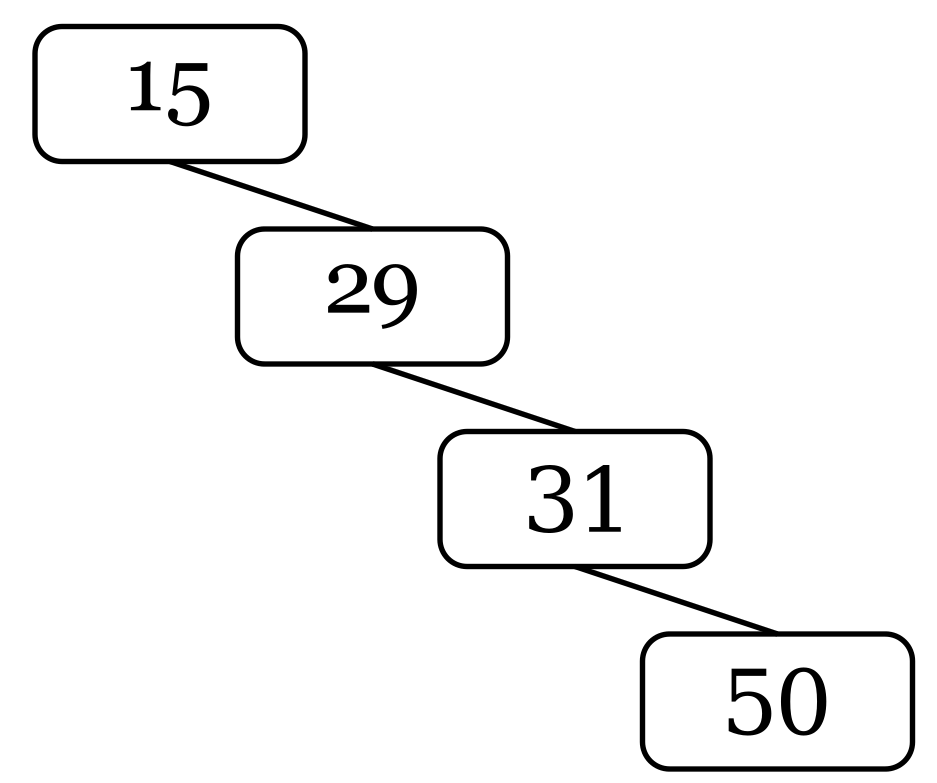
\includegraphics[scale=0.15]{../../media/linear.png}
          \end{center}
    \item Die Sortierung in der Baumstruktur wird noch einmal deutlich, wenn man folgendes Bild betrachtet:
          \begin{center}
              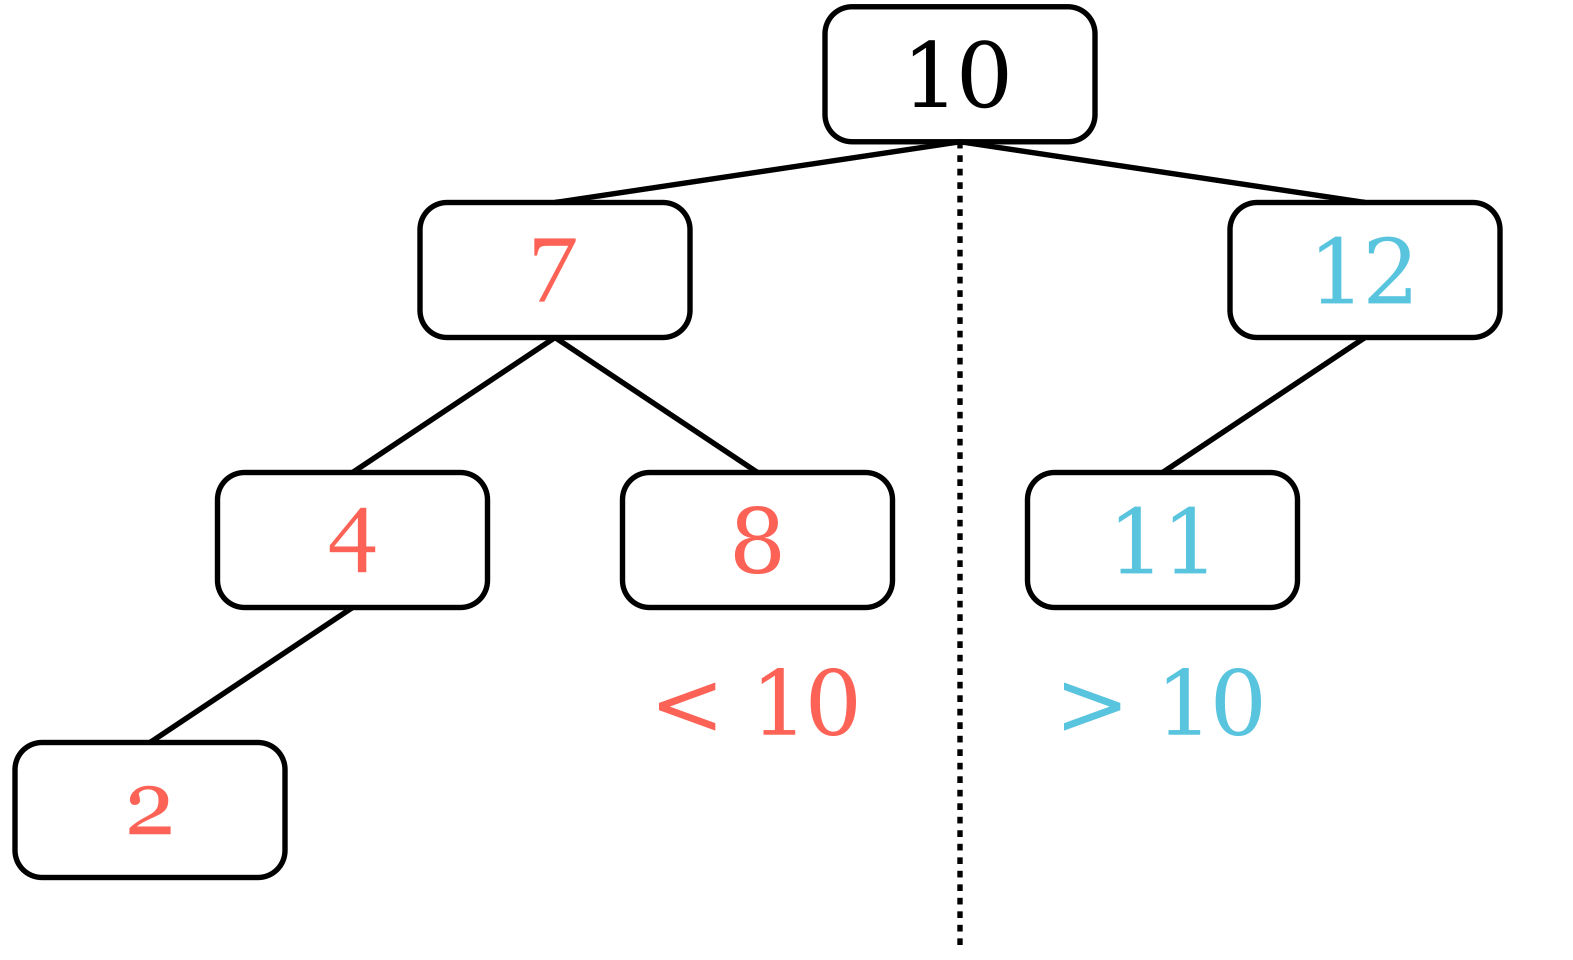
\includegraphics[scale=0.15]{../../media/sortedTree.png}
          \end{center}
          Zieht man eine Linie senkrecht unterhalb eines beliebigen Knotens, so sind alle Knoten im linken Teilbaum kleiner und alle Knoten im rechten Teilbaum größer.
\end{itemize}

\begin{task}{Einfügen}
Zeichnen Sie jeweils schrittweise den binären Suchbaum, der sich ergibt, wenn die folgenden Zahlen in der gegebenen Folge eingefügt werden. \\
\textbf{a)} $5 \rightarrow 7 \rightarrow 3 \rightarrow 2 \rightarrow 4 \rightarrow 6 \rightarrow 10 \rightarrow 11$ \\
\textbf{b)} $10 \rightarrow 11 \rightarrow 5\rightarrow 7 \rightarrow 6 \rightarrow 4 \rightarrow 3 \rightarrow 2$
\end{task}
Und jetzt auf zur Implementierung!
\end{document}